\subsubsection{Salīdzinājums} \label{sec:fast-compare}
Iepriekš apskatīto implementāciju salīdzināšana nav triviāls uzdevums.
Pat salīdzinot tikai CPU implementācijas (sk.~pielikumu~\ref{appx:test1}),
tika iegūti nekonsistenti rezultāti, kas atspoguļoti
\ref{fig:test1-data-txt}~attēlā.
\begin{figure}[tbh]
	\centering
	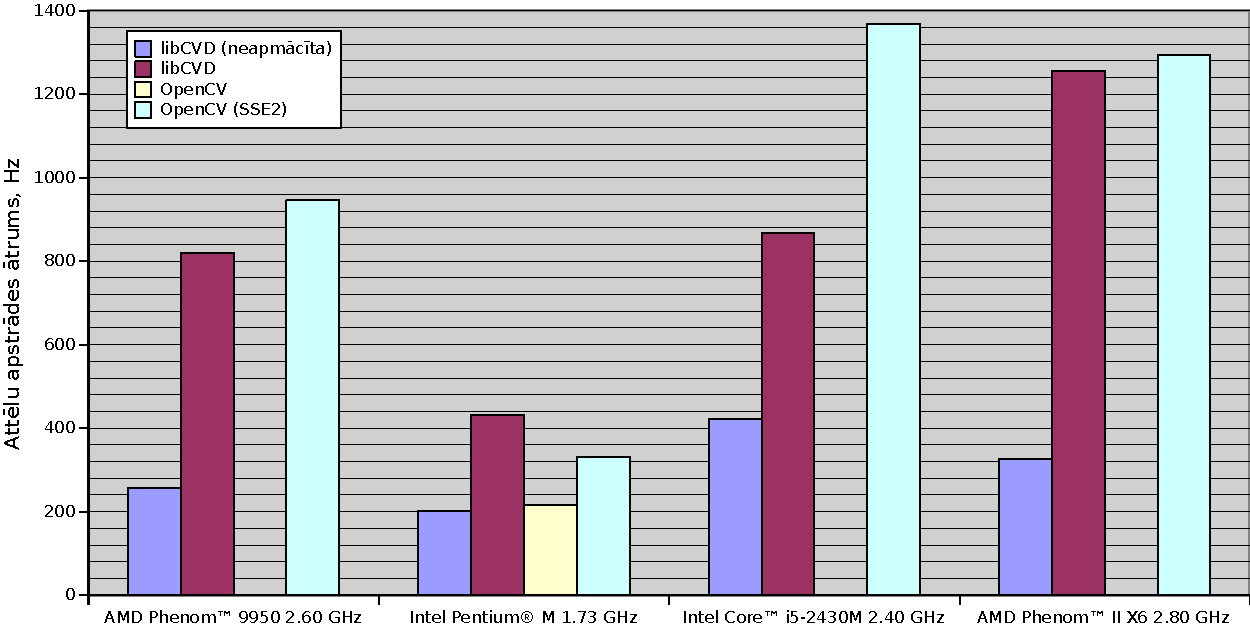
\includegraphics[width=\linewidth]{chart-cpu2}
	\caption{FAST CPU implementāciju ātrdarbības salīdzinājums.}
	\label{fig:test1-data-txt}
\end{figure}

Vecākas paaudzes Pentium procesoram labākais ātrdarbības rādītājs bija tieši
mašīnmācāmajai (libCVD) FAST implementācijai, savukārt jaunāko paaudžu
procesoriem labāku ātrdarbību uzrādīja OpenCV SSE2 uzlabotā implementācija.
AMD~Phenom~II gadījumā libCVD un OpenCV SSE2 implementācijas uzrādīja
līdzvērtīgu rezultātu.
Šādi rezultāti skaidrojami, galvenokārt, ar SSE2 veiktspējas uzlabojumiem
jauno paaudžu procesoriem~\cite{Core2}. Papildus tam, mašīnmācāmā FAST
implementācijas jautājumu koks veido apjomīgu mašīnkodu ar lielu skaitu
zarošanos. Koda apjoms un nelineārā izpildes secība samazina izpildes koda
lokalitāti un ierobežo instrukciju kešatmiņas efektivitāti.

\ref{fig:test1-data-txt}~attēlā OpenCV (bez SSE2) rezultāti 64~bitu
sistēmām nav uzrādīti, jo kompilācijas sistēma nerespektēja (ignorēja)
SSE2 atspējošanu un iegūtie rezultāti bija nekorekti
(\ref{fig:test1-data}~attēls \pageref{fig:test1-data}~lapā iekļauj arī nekorektos
rezultātus).

GPU implementācijas ātrdarbība tika salīdzināta ar CPU platformu,
kas uzrādīja līdzīgus rezultātus ar CPU implementāciju, bet tos
nepārsniedzot, kā tika paredzēts (sk.~\ref{fig:test2-data-txt}~att.).
Autors šo veiktspējas
ierobežojumu skaidro ar salīdzinoši mazo datu apjomu un
zemu nepieciešamo skaitļošanas apjomu. Tādējādi GPU straumes
procesori nav pietiekami piesātināti ar datiem, kā rezultātā tie
procentuāli daudz laika pavada dīkstāvē un
GPU augstais latentums ir galvenais ierobežojošais faktors.
(GPU arhitektūra apskatīta \ref{sec:gpu}~nodaļā).
\begin{figure}[tbh]
	\centering
	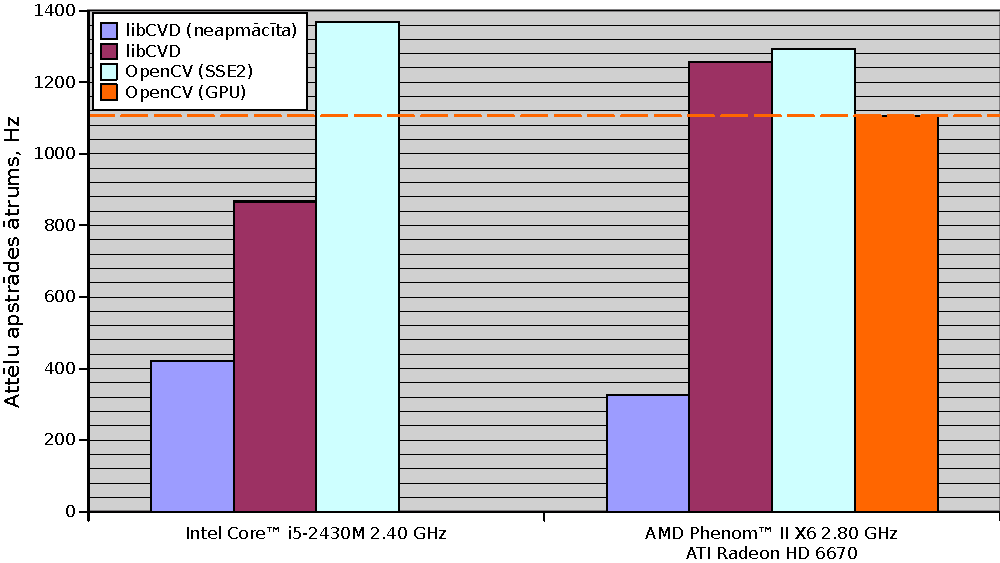
\includegraphics[scale=0.77]{chart-gpu2}
	\caption{FAST GPU un CPU implementāciju ātrdarbības salīdzinājums.}
	\label{fig:test2-data-txt}
\end{figure}

Autora izstrādātais FPGA implementācijas modelis tika sintezēts ar
dažādu skaitu punktu apstrādes vienību un to veiktspēja aprēķināta
ņemot vērā sintēzes rezultātos iegūto maksimālo frekvenci.
Testos novērots, ka $12 \times 12$ pikseļu gabala apstrāde pie
aptuveni $400\units{MHz}$ takts frekvences sasniedz CPU platformas
labākos rezultātus.
Rezultāti ilustrēti \ref{fig:test3-data-txt}~attēlā, kur ar
melnu, pārtrauktu līniju atzīmēts labākais
CPU implementācijas rezultāts. Ātrdarbība FPGA ir palielināma
instancējot vairāk punktu apstrādes vienību.

\begin{figure}[tbh]
	\centering
	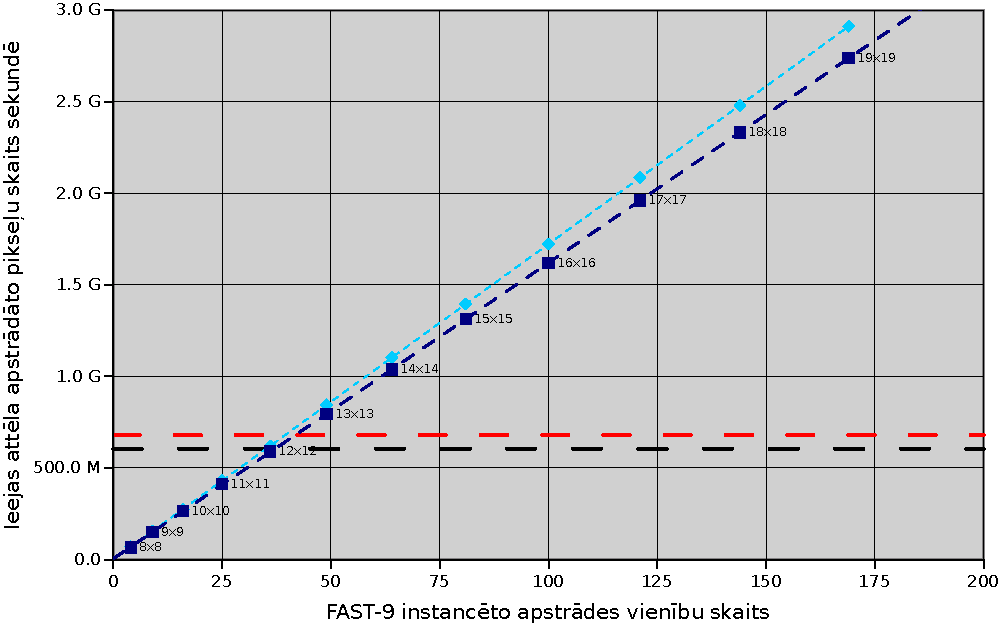
\includegraphics[scale=0.77]{chart-fpga}
	\caption{Pikseļu apstrādes ātrums pret \texttt{fast\_n\_unit} instanču skaitu.}
	\label{fig:test3-data-txt}
\end{figure}

Kopumā, FAST implementācija FPGA uzrādīja augstāko potenciālo ātrdarbību,
aiz kuras seko CPU. GPU uzrādīja līdzīgu rezultātu kā CPU, bet tests ar
vienu ierīci nevar adekvāti vispārēji atspoguļot GPU platformas veiktspēju.
Autors arī uzsver,
ka pat ja GPU implementācija uzrāda zemāku ātrdarbību nekā CPU, tā
izmantošana tomēr var palielināt kopējo (heterogēnas) sistēmas ātrdarbību
atslogojot CPU, gadījumos, ja tam jāveic papildus skaitļošanas uzdevumi.
Visu pārbaudīto ierīču ātrdarbība ievērojami pārsniedza
30~kadrus sekundē ($768 \times 576$ pikseļu lielam kadram) 
un tās ir izmantojamas reāllaika datu
straumes apstrādei. 30~kadri sekundē gan nav mērķis, bet minimums, jo
raksturpunktu detektēšana ir tikai viens solis, un lai nodrošinātu
pietiekamu apstrādes laiku visam uzdevumam, šis rādītājs ir jāpārsniedz
vairākas reizes.
